%!TEX root=document.tex


\subsection{Custom Execution Engine}
\label{sec:in_memory_execution_engine}

From our implementation of the DBMS-backed execution engine, 
we learned that its design suffers from two drawbacks:
(a) the number of scans performed of the data is far too high, and
(b) far too many resources are wasted on low-utility views.
As a result, our goals with the custom execution engine are as follows:
(a) complete sharing of table scans between views so that a single table scan
suffices to compute all views; 
(b) sharing of intermediate results between views so that low utility views can
be pruned on the fly; and 
(c) early stopping once the top views have been identified. 
We now describe the
basic execution framework adopted by our engine followed by specific
pruning strategies.

\subsubsection{Basic Framework}
\label{subsec:basic_framework}
Algorithm~\ref{algo:custom_exec_engine} in the appendix shows the basic framework adopted by our
custom execution engine.
\VizRecDB\ buffers data from the input file (on disk or in memory) and processes it
one record at a time.
We assume that {\it records in the file are in random order}; if they are not,
we must apply a pre-processing step to get them in random order.
For each record read in, \VizRecDB\ determines whether the record satisfies the
input query, and then updates the target and comparison views for all views
currently in the running or have been ``accepted'' as being in the top-$k$.
It also updates the utility values and other algorithm-specific statistics for
each view.
To avoid doing expensive pruning computations after reading each record,
\VizRecDB processes the file in phases where each phase consists of processing a
fixed number of records.
At the end of a phase, \VizRecDB\ checks to see if any views can be pruned,
i.e., discarded, or accepted as being in the top-$k$.
% At one extreme, each phase consists of just one record, in which case views
% are pruned after ever record is read and the views are updated;
% at the other extreme, we use only one phase, in which case views are only pruned
% after all the records are read (i.e., effectively no pruning). 
The list of views in the running is updated and processing continues.
Once we meet a pre-defined stopping criteria, $k$ views with the
highest utility are returned to the frontend.
We implement two stopping criteria: we either stop once the entire table has
been processed (and return exact views to the user), or we stop after
we have ``accepted'' $k$ views as being in the top-$k$ (and return
approximations of the top-$k$ views to the user).
We use the former as the default stopping condition.

% Note that we have two alternatives for computing the visualizations for the top-$k$
% views, once $k$ views have been accepted: 
% we can either compute the top-$k$ views to completion (i.e.,
% on the remaining unprocessed records),
% or we can display approximate visualizations for each view, as soon as we ``accept'' them
% as being in the top-$k$. 
% We use the former option as the default, 
% and the latter as an additional optimization that may be employed.
% If at the end of a given phase, \VizRecDB\ finds that the views in running satisfy
% the given stopping criteria, e.g., that \VizRecDB\ has already identified the
% top-$k$ views, the \VizRecDB\ engine can stop processing early.

% \begin{algorithm}
% \caption {ComputeAggregate(Query
% {\it currQuery}, int $d$)}
% %\small 
% \begin{algorithmic}[1] 
% \State int[$d+1$] $currCard$\ \ //All arrays are
% indexed from 1 
% \STATE $currCard[1]$ = ExecuteCellQuery({\it currQuery})  
% \FOR {$i=2$ to $d+1$} 
% \STATE {\it prevQuery} $\leftarrow$ GetPreviousNeighbour($i$-1)\ \ //decrement
% the $(i-1)^{th}$ dimension of {\it currQuery} by stepsize 
% \STATE int[] $prevCard$ = GetAllAggregates({\it prevQuery})
% \STATE $currCard[i]$ = $currCard[i-1]$ + $prevCard[i]$ 
% \ENDFOR 
% \STATE StoreAllAggregates({\it currQuery}, $currCard$) 
% \STATE {\bf return} $currCard[d+1]$
% \end{algorithmic}
% \label{algo:aggregatecomputation}
% \end {algorithm}




The general idea is to keep running estimates of utility for each view, and
perform pruning of low utility views based on these estimates.
To implement a pruning strategy, we merely specify two things: (1)
statistics to track for each view, and 
(2) the rule used to prune views at the end of a phase.
% An important side effect of our implementation is that
% as we scan more data from the file, our estimates of utilities become more
% accurate.
In this paper, we propose and evaluate three different strategies
to perform the pruning of views. The first two
strategies are based on top-$k$ algorithms that use confidence intervals, and
the third is based on an adaptation of the Multi-Armed Bandit problem to our
setting.
% 
% \begin{itemize}
% \item The first two strategies are based on confidence interval-based top-$k$ algorithms.
% That is, at the end of each phase, confidence intervals are updated for all
% the views still in the running and we prune views based on overlap
% with the top-$k$ confidence intervals.
% % and if the upper-bound for any of them
% % is lower than the lower-bound for confidence intervals of $k$ or more other views,
% % then those views are discarded.
% \begin{denselist}
% \item The first uses worst-case confidence intervals based on the
% Hoeff\-ding-Serfling inequality~\cite{serfling1974probability}, 
% which is a generalization of Hoeffding's inequality~\cite{hoeffding1963probability}
% when a number of samples are randomly chosen without replacement
% from the same set.
% These confidence intervals are necessarily more conservative.
% \item The second assumes that the underlying probability distribution is
% Gaussian and uses 95\% confidence intervals~\cite{all-of-statistics}.
% These confidence intervals are more ``aggressive'' compared to those derived
% from the Hoeffding inequality.
% (For experiments evaluating this assumption, see Section~\ref{sec:evaluating_normal}.) 
% \end{denselist}
% \item The last strategy is based on an adaptation of Multi-Armed Bandit (MAB)
% algorithms for top-$k$ arm identification~\cite{}. 
% Multi-Armed Bandit algorithms are well-studied in the field of stochastic
% control; in our scenario, the arms are the views, and pulling an arm corresponds
% to updating a view's utility.
% \end{itemize}


\subsubsection{Confidence Interval-Based Pruning}
\label{sec:confidence_interval}
We first describe at a high-level our confidence interval-based pruning strategies,
and then describe the two specific instantiations of these strategies,
based on worst-case, and normal confidence intervals respectively.

Confidence Interval-based pruning works as follows: at every step of our
algorithm, we keep an estimate of the mean utility for every view and a
confidence interval around that mean.
That is, for every view $V_i$ we track its mean utility $u_i$, and a
confidence interval around the mean, $u_i \pm c_i$.
At the end of a phase, we use the following rule to prune low-utility
views:
{\em If the upper bound of the utility of view $V_i$ is lesser
than the lower bound of the utility of $k$ or more views, then $V_i$ is discarded.}

\begin{figure}[h]
\vspace{-10pt}
\centerline{
\hbox{\resizebox{9cm}{!}{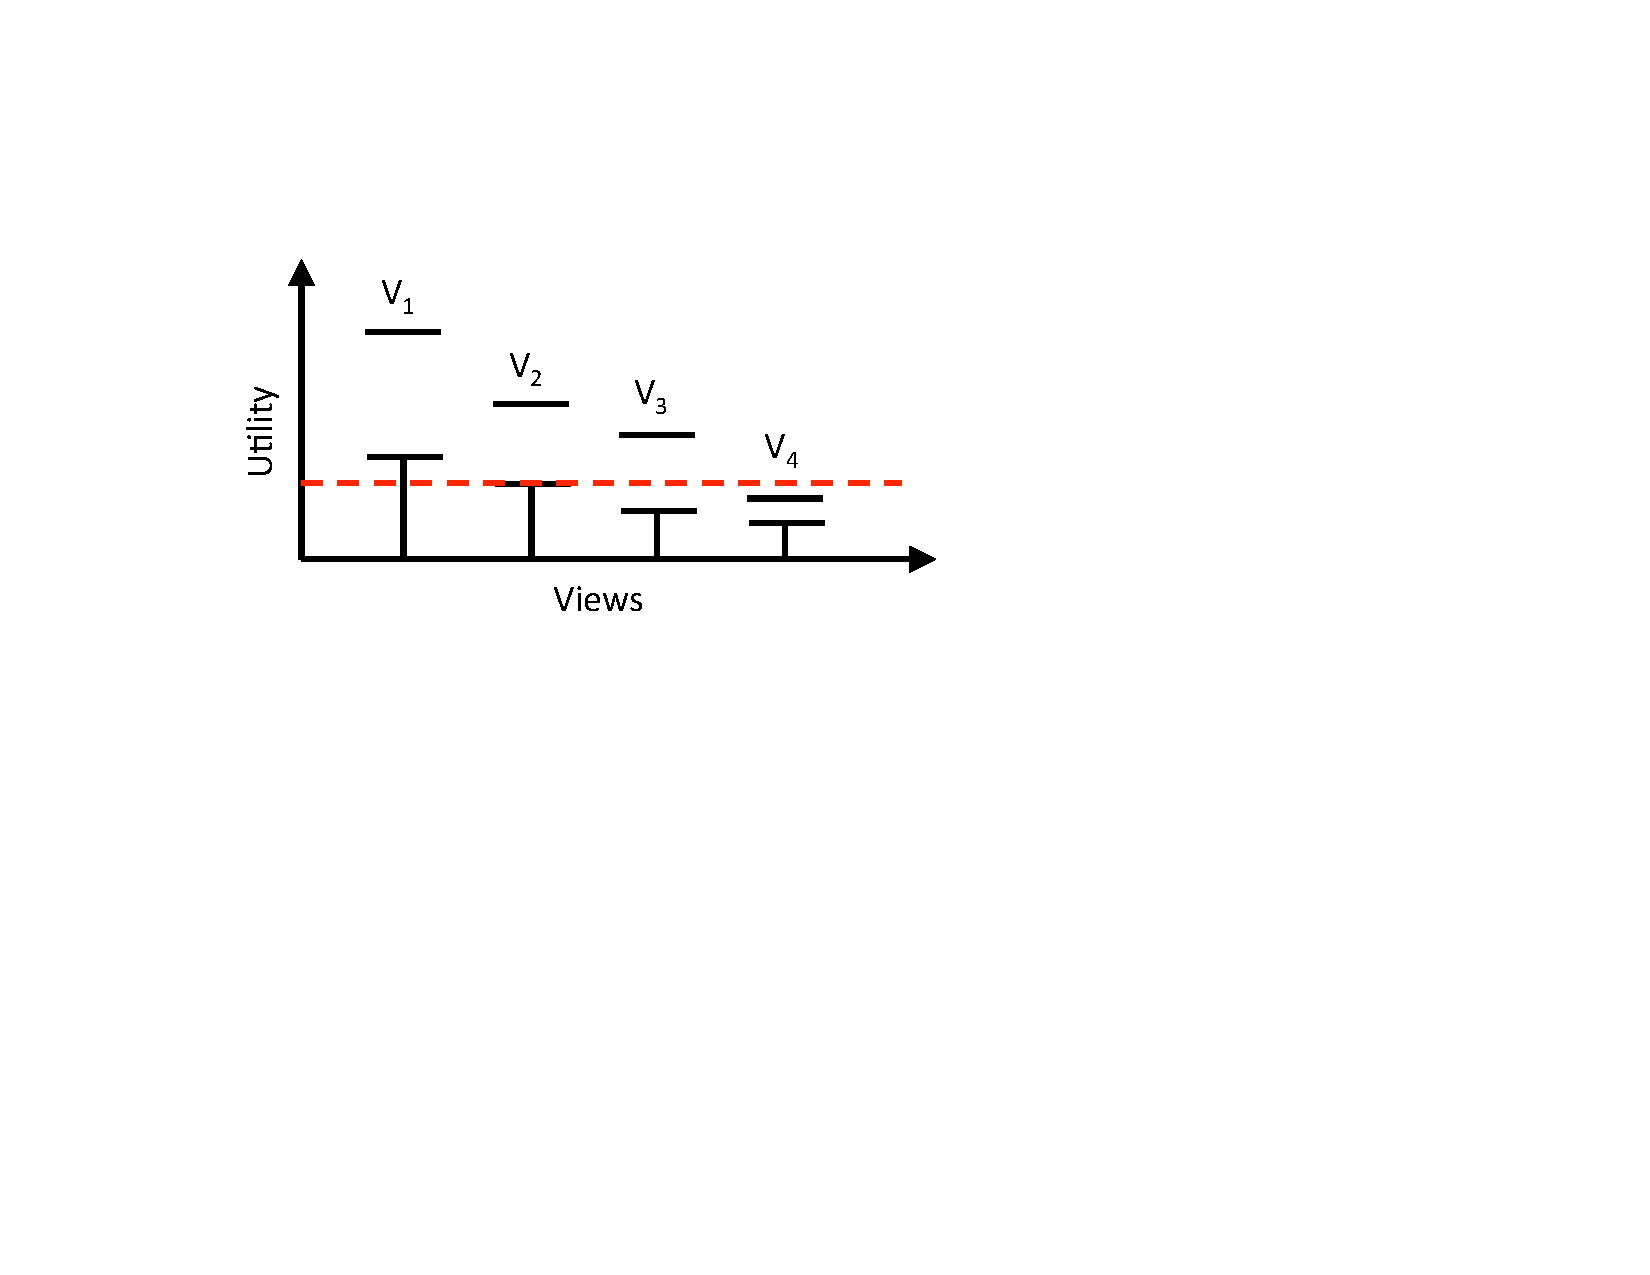
\includegraphics[trim=10mm 100mm 55mm 35mm, 
clip=true]{Images/confidence_pruning.pdf}}}}
\vspace{-20pt}
\caption{Confidence Interval based Pruning}
\label{fig:conf_interval}
\vspace{-15pt}
\end{figure}

We illustrate this with an example. Suppose a dataset has 4 views $V_1$
to $V_4$ and we want to find the top-$2$ views.
Further suppose that at the end of phase $p$,
$V_1$-$V_4$ have confidence intervals as shown in Figure \ref{fig:conf_interval}.
Views $V_1$ and $V_2$ have the highest estimates for utility so far.
Consider view $V_3$; we see that its confidence interval overlaps with the
confidence intervals of the current top views, making it possible
that $V_3$ will be in the final top views. On the other hand, the confidence
interval for $V_4$ lies entirely below the lowerbounds of $V_1$ and $V_2$.
Since we can claim with high probability (depending on the confidence threshold)
that the utility of $V_4$ lies within its confidence interval, it follows that
with high probability, $V_4$'s utility will be lower than that of both $V_1$ and
$V_2$, and it will not appear in the top-$2$ views.
This is our pruning rule. 
We state the algorithm fomally in
Algorithm~\ref{algo:ci_based_pruning} in the appendix.

Next, we discuss two confidence interval computation techniques.


\stitle{Worst-Case Confidence Intervals.} 
Suppose we have $N$ values $y_1, \ldots, y_n$ in $[0, 1]$, and we are drawing
from them without replacement. 
Say we have drawn $m$ values so far, which are $Y_1, \ldots, Y_m$.
Then, we use the Hoeffding-Serfling inequality~\cite{serfling1974probability} 
to derive a running 
confidence interval around the current mean 
of the $m$ values such that the actual mean of the $N$
is always within this confidence interval with a probability of $1 - \delta$:
\begin{theorem}
\label{thm:hs}
Let $\calY = y_1,$ $\ldots,$ $y_N$ be a set of $N$ 
values in $[0,1]$ with average value
$\frac1N \sum_{i=1}^N y_i = \mu$.
Let $Y_1,\ldots,Y_N$ be a 
sequence of random variables drawn from $\calY$ without
replacement.
Fix any $\delta > 0$. For $1 \le m \le N-1$, define
$$
\varepsilon_m = \sqrt{\frac{(1-\frac{m-1}N)(2\log \log (m) + \log(\pi^2/3\delta))}{2m}}.
$$
$$
\textrm{Then:} \ \   \Pr\left[ \exists m, 1 \le m \le N : 
  \left|\frac{\sum_{i=1}^m Y_i}{m} - \mu\right| > \varepsilon_m \right] 
\le \delta.
$$

\end{theorem}
In our setting, the current mean, $\sum Y_i / m$, is the 
the current estimate of the utility of a view 
based on the entire set of records seen thus far. 
Therefore, to apply this pruning strategy, the only statistics
we track are the current estimates of view utilities.

Note that in this setting, we are assuming that since the
utility estimate at any stage of processing is in $[0, 1]$, 
the $Y_i$ values, i.e., the incremental contributions to the utility
that come from reading each record, are also between $[0, 1]$,
and are independent of the current value of the utility. 
This is is not true in our setting, 
because the utility function could be arbitrary.
Thus, the theoretical guarantees do not directly apply to our setting. 

\stitle{Normal Confidence Intervals.} In this scheme, we assume that the utility
distributions for each view are Gaussian and apply the standard confidence
intervals to our utility measurements.
% We describe the equations first assuming that
% when every time a record is read, for every view,
% a utility value is ``sampled''
% from a normal distribution. (This assumption is not
% quite correct; we will discuss this  below.)

Consider a specific view $V_i$. 
If the mean utility across the sampled records 
(i.e., the records read thus far) is $\mu$,
and the variance in the utility of the sampled records
is $\sigma$, then, we have:
\begin{align}
CI & = \mu \pm z \times \frac{\sigma}{\sqrt{m}}
\end{align}
Thus, the CI (or confidence interval) is 
a confidence interval centered around $\mu$, 
and depends on $\sigma$. 
It additionally depends on the number of records
read thus far, $m$,
and $z$, the factor that depends on our confidence interval threshold.
For instance, for a 95\% confidence interval, $z = 1.96$.

We note that the assumption that we are drawing from a normal distribution is
not quite accurate since our samples vary in size and are not independent.
As a result, we make two simple adjustments to the confidence interval
calculations that are described in Appendix~\ref{sec:ci_pruning}.
In Section \ref{sec:experiments}, we show experimentally on multiple datasets
that our confidence interval calculations accurately capture utility and can be used to
perform pruning with high confidence.






% \stitle{Normal Confidence Intervals.}
% As described above, we must specify
% a set of statistics to track for each view and a rule that is used to
% prune views based on the statistic.
% For confidence interval based pruning, the statistics we track are the mean, 
% variance, and confidence intervals of the view utility.
% As \VizRecDB\ reads each record, it updates the data
% distributions for all views and calculates the current utility of each view. 
% Using past measures of utility, \VizRecDB\ also tracks the mean,
% variance and confidence intervals for the utility of each view.
% % At the end of a phase, \VizRecDB\ uses the following rule for pruning low-utility
% % views (stated more formally below): {\it if the upperbound on the utility
% % of view $v_i$ is lesser than the least lowerbound on the utility of the
% % top-$k$ views, view $v_i$ is discarded.}

% % Let us dive deeper into this pruning rule.
% Note that as we sequentially read records from a file, we are
% approximating a sampling process (remember that the records are in random order).
% For instance, suppose that we have read 10K records from a 1M record file.
% In this case, the records 1 -- 10K constitute a 1\% sample of the entire file.
% When we read the next say 10 records, the records 1 -- 10,010 constitute an
% incrementally larger sample of the underlying file.
% Thus, as we read more data from the file, we obtaining a large
% number of samples from the underlying data (notice however, that these samples
% are not independent).

% Since we are generating a large number of samples from a population, we can
% invoke a well-studied concept in statistics called the ``sampling distribution.'' 
% A sampling distribution for a statistic $S$ is the distribution of
% $S$ generated by taking a large number of samples of a fixed size and computing
% the statistic $S$ on each sample.
% In our case, the population we draw from is the set of all records in the file
% and our samples are the increasingly larger sets of records that we are reading in.
% The statistic $S$ that we are computing is the view utility (we
% compute a utility value for each view).
% Now, the sampling distribution of the {\it mean} has been well studied and it
% has been proven that the mean of the sampling distribution is equal to the mean of the
% population and the standard error of the sampling distribution is equal to the
% standard error of the population divided by the square root of the sample size. 
% These two formulas are shown in Equations \ref{eq:mean} and \ref{eq:variance}.
% Similarly, if we know the mean and standard error of the sampling distribution,
% we can compute a confidence interval around the population mean. This is shown
% in Equation \ref{eq:confidence_interval} where $z$ is the factor that depends on the
% confidence threshold we are aiming for and $N$ is the number of items
% in each sample.

% \begin{eqnarray}
% \label{eqnarray:mean_and_variance}
% \mu_M = \mu \label{eq:mean}\\
% \sigma_{M} = \frac{\sigma}{\sqrt{N}} \label{eq:variance}\\
% CI = \mu_M \pm z \ast \frac{\sigma_M}{\sqrt{N}}\label{eq:confidence_interval}
% \end{eqnarray}

% If we were modeling the mean of our samples instead of the utility, we could use
% the above result directly.
% However, we find that with a few minor modifications, we can use the confidence
% interval bounds shown above.
% The first modification we make has to do with how we define utility.
% Remember from Section \ref{sec:problem_definition} that the utility of a view is
% defined as the distance between two distributions: the distribution of aggregate values for the
% target view and the distribution of aggregate values for the comparison view.
% These distributions are in turn tied to the number of distinct groups present in
% each dimension attribute.
% For our purposes, it means that if a dimension attribute has $n$ distinct
% groups, then a sample with $x$ rows gives us approximately $\frac{x}{n}$ values
% for each group (assuming uniform distribution).
% Said another way, a sample with $x$ rows for the purpose of computing utility is
% really only a sample of $\frac{x}{n}$ rows.
% So the first modification we make to Equation \ref{eq:confidence_interval} is to
% replace $N$ by $\frac{N}{G_{max}}$ where $G_{max}$ is the maximum number of
% distinct groups present in any dimension attribute.
% Second, we observe that the sampling distribution applies to the case where
% samples are of the same size and are independently generated.
% This is not true in our algorithm; therefore, to compensate, make two
% conservative modifications: we set $N$ to the number of rows that
% have been read in the previous phase (remember that pruning happens at the end
% of every phase) and we set the $z$ parameter to a value $\geq$ 1.96 (the normal
% 95\% confidence interval value). These modifications ensure (as we will show
% empirically in Section \ref{sec:experiments}) that the confidence intervals
% always contain the mean and continually shrink as we read in more data.

% As shown in Line 12 of Algorithm \ref{algo:custom_exec_engine},
% when a phase ends, we clear all statistics collected in that phase; we do not
% want less accurate estimates from previous phases to contaminate the more
% accurate estimates from subsequent phases. \agp{deal with this.}






% Now that we have a way of finding confidence intervals, we elaborate on how we
% use them to perfom pruning.
% Suppose at the end of phase $p$ the confidence intervals for the views in
% running have values shown in Figure \ref{fig:conf_interval} and we want to
% identify the two views with the highest utility.
% Consider view $V_3$, we see that its confidence interval overlaps with the
% confidence intervals of the current top views $V_1$ and $V_2$, making it likely
% that $V_3$ will be in the final top views. On the other hand, the confidence
% interval for $V_4$ lies entirely below the lowest bound of the top two
% intervals.
% Since we can claim with high probability (depending on the confidence threshold)
% that the utility of $V_4$ lies within its confidence interval, it follows that
% with high probability, $V_4$ will not appear in the top-$2$ views.
% This is essentially our pruning rule. 
% 



\subsubsection{Multi-Armed Bandit Pruning}
\label{sec:multi_armed_bandit}
The second class of pruning techniques we explore
are based on solutions for Multi-Armed Bandit (MAB), a problem 
in stochastic control. 
The setting is as follows: 
a gambler is faced with several slot
machines (``arms'') that each have an underlying reward
distribution. 
At each turn, the gambler must decide which machine
to play at; when they play the machine, they get a reward.
The gambler needs to decide on a {\em strategy}, i.e.,
which machine to play during every turn, to maximize
eventual, total, or time-decaying rewards~\cite{bandits}.
Recently, variants of MAB have been proposed 
which instead of maximizing total reward, 
focus on finding the arms with the highest mean reward~\cite{BubeckWV13}.
This is very similar to our setting: each possible view can be thought of as
one arm and our goal is find the views with the highest reward (i.e.
utility).
In MAB, each pull of an arm corresponds to a drawing from a sample
the underlying probability distribution of that arm.
In our case, each new record updates the utilities for all views and
each resulting updated utility can be thought of as a sample from the
utility distribution of that view.
There are two approximations we make here to apply MAB techniques
to our setting: 
(1) although the utility of a
view is ultimately a single value, we can approximate it as a probability
distribution that is normally distributed around the true utility, and 
(2) our running estimate of utility after reading $i$
records is a sample derived from the above utility distribution.
As we show in our evaluation, the approximation works well
for our purposes.

Algorithm~\ref{algo:mab_based_pruning} (in the appendix) shows the pruning technique used in the
MAB setting.
This algorithm is an adaptation of the Successive Accepts and Rejects
algorithm from \cite{BubeckWV13} for finding the top-$k$ arms with the highest
mean reward.
As before, the processing of the whole file is divided into phases.
% As opposed to the confidence interval technique, we only track a single
% statistic for MAB, namely the utility mean.
At the end of every phase, we adopt the following pruning technique: all views
in running are ranked in order of their utility means. 
We then compute two special differences between the utility means: $\Delta_1$
is the difference between the highest mean and the $k+1$st highest mean, and
$\Delta_n$ is the difference between the lowest mean and the $k$th highest mean.
If $\Delta_1$ is greater than $\Delta_n$, the view with the highest mean is
``accepted'' as being part of the the top-$k$ (and it no longer participates
in pruning computations).
On the other hand, if $\Delta_n$ is higher, the view with the lowest mean is discarded
from the set of views in the running.




% \techreport{\cite{BubeckWV13} provides bounds on the optimality of this heuristic for the
% MAB setting.
% Since our problem setup isn't exactly the same, the optimality bounds don't
% transfer directly.
% However, as we show in the experimental section, the MAB heuristic performs well
% on real datasets.}